\documentclass{beamer}
\mode<presentation>
\title{Free and Open Source Software}
\author{Andrea Bellandi, Alessandro Campagni}
\usetheme{CambridgeUS}


\begin{document}


\begin{frame}
  \titlepage

\vfill

\includegraphics[width=0.05\textwidth]{img/cc.png}
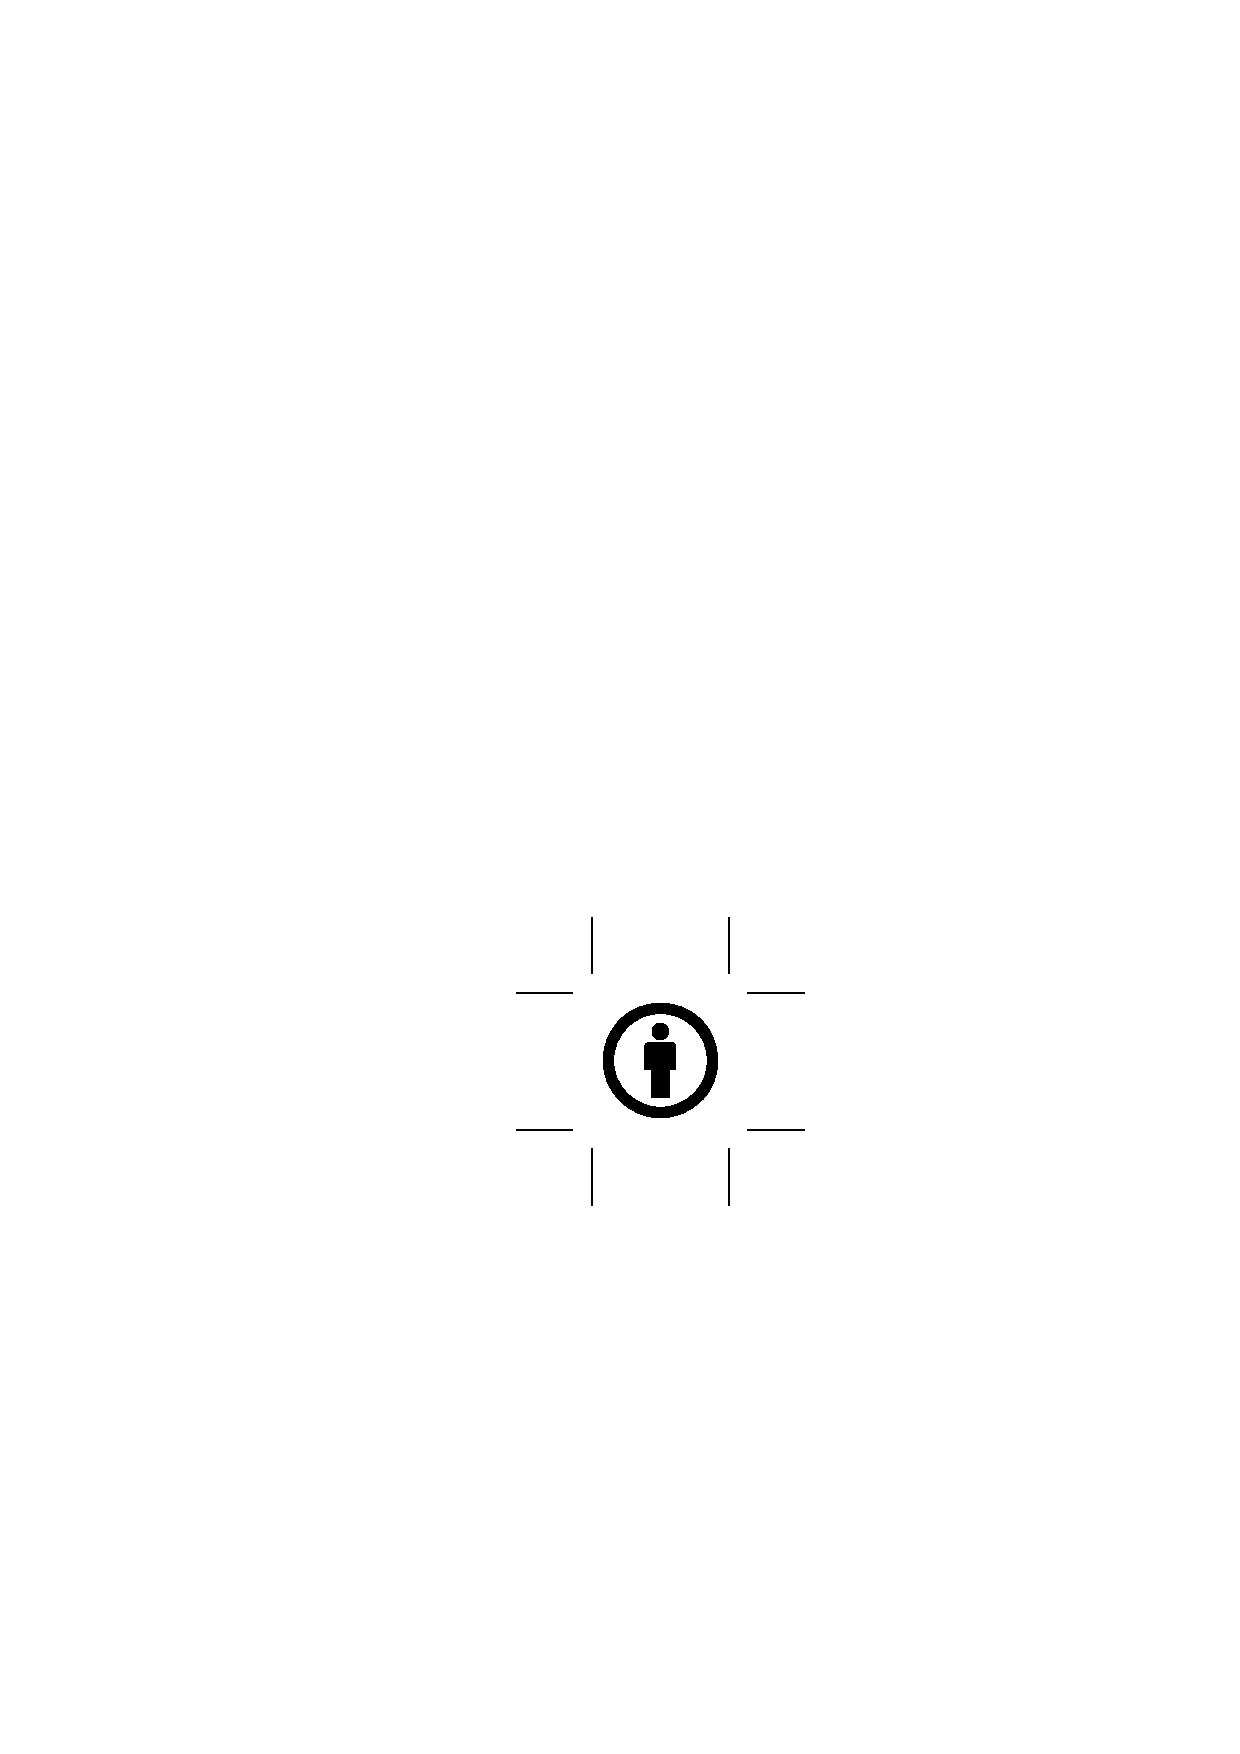
\includegraphics[width=0.05\textwidth]{img/by.png}

\includegraphics[width=0.05\textwidth]{img/sa.png}

This work is licensed under the Creative Commons Attribution-ShareAlike 3.0 Unported License. To view a copy of this license, visit http://creativecommons.org/licenses/by-sa/3.0/.
\end{frame}

\begin{frame}
  \frametitle{Free and Open Source Software}

  \begin{itemize}
    \item Cosa \`e il FOSS
  \end{itemize}

\end{frame}


\begin{frame}
  \frametitle{Cosa \`e il FOSS}
Qui direi due paroline su cos'\`e il software libero, sulle licenze,
le quattro libert\`a ecc...
\end{frame}

\begin{frame}
  \frametitle{Free and Open Source Software}

  \begin{itemize}
    \item Cosa \`e il FOSS
    \item Perch\'e il FOSS
  \end{itemize}

\end{frame}

\begin{frame}
  \frametitle{Perch\'e il FOSS}
Enfatizzare sulle quattro libert\`a come risposta al perch\`e, magari
facendo un esempio su cosa accadesse se i teoremi della matematica
(visto che la platea \`e di matematici) fossero chiusi! Magari parlare
di possibilit\`a di riuso del codice, e altri vantaggi che si hanno ad
avere i sorgenti.
\end{frame}

\begin{frame}
  \frametitle{Free and Open Source Software}

  \begin{itemize}
    \item Cosa \`e il FOSS
    \item Perch\'e il FOSS
    \item Ma allora conviene
  \end{itemize}

\end{frame}

\begin{frame}
  \frametitle{Ma allora conviene}
Continuare ad enfatizzare ancora sulle quattro libert\`a: il vero
motivo di convenienza del FOSS, e ricordare che free non significa che
non ti devo far pagare!
\end{frame}

\end{document}
